%This is a LaTeX template for homework assignments
\documentclass[8pt]{article}
\usepackage[top=1in, bottom=1in, left=1.1in, right=1.1in]{geometry}
\usepackage[utf8]{inputenc}
\usepackage{amsmath}
\usepackage{CJK}
\usepackage{enumerate}
\usepackage{ifthen}
\usepackage{listings}
\lstset{
  language=python,
  keywordstyle=\color{blue!70},
  frame=single,
  basicstyle=\ttfamily,
  commentstyle=\color{red},
  breakindent=0pt,
  rulesepcolor=\color{red!20!green!20!blue!20},
  rulecolor=\color{black},
  tabsize=4,
  numbersep=5pt,
  showstringspaces=false,
  breaklines=true,
  backgroundcolor=\color{red!10},
  showspaces=false,
  showtabs=false,
  extendedchars=false,
  escapeinside=``,
  frame=no,
}

\usepackage{fourier}
\usepackage{pgf}
\usepackage{tikz}
\usetikzlibrary{calc}
\usetikzlibrary{arrows,snakes,backgrounds,shapes,shadows}
\usetikzlibrary{matrix,fit,positioning,decorations.pathmorphing}



\newcommand{\tf}{\ttfamily}


\newlength{\la}
\newlength{\lb}
\newlength{\lc}
\newlength{\ld}
\newlength{\lhalf}
\newlength{\lquarter}
\newlength{\lmax}
\newcommand{\xx}[4]{\\[.5pt]%
\settowidth{\la}{A.~#1~~}
\settowidth{\lb}{B.~#2~~}
\settowidth{\lc}{C.~#3~~}
\settowidth{\ld}{D.~#4~~}
%%
\ifthenelse{\lengthtest{\la>\lb}}
{\setlength{\lmax}{\la}}
{\setlength{\lmax}{\lb}}
\ifthenelse{\lengthtest{\lmax<\lc}}
{\setlength{\lmax}{\lc}}
{}
\ifthenelse{\lengthtest{\lmax<\ld}}
{\setlength{\lmax}{\ld}}
{}
%%
\setlength{\lhalf}{0.5\linewidth}
\setlength{\lquarter}{0.25\linewidth}
%%
\ifthenelse{\lengthtest{\lmax>\lhalf}}
{\noindent{}A.~#1 \\ B.~#2 \\ C.~#3 \\ D.~#4 }
{
\ifthenelse{\lengthtest{\lmax>\lquarter}}
{\noindent
\makebox[\lhalf][l]{A.~#1~~}%
\makebox[\lhalf][l]{B.~#2~~}\\
\makebox[\lhalf][l]{C.~#3~~}%
\makebox[\lhalf][l]{D.~#4~~}
}%
{\noindent
\makebox[\lquarter][l]{A.~#1~~}%
\makebox[\lquarter][l]{B.~#2~~}%
\makebox[\lquarter][l]{C.~#3~~}%
\makebox[\lquarter][l]{D.~#4~~}
}
}
}



\begin{document}
\begin{CJK}{UTF8}{gkai}
\begin{center}
{\Large \bf  武汉大学数学与统计学院2017-2018学年第一学期期末考试\\[0.1in]
  数据结构与算法(A卷)} \vspace{0.1in}

姓名: \line(1,0){100} ~~~~~~ 学号: \line(1,0){100}

\end{center}


\begin{enumerate} %\line(1,0){20}
\item (20分)~Python相关
  \begin{enumerate}
  \item 给定长(\lstinline{length})和宽(\lstinline{width}),编写长方形(\lstinline{Rectangle})的类,并求其面积和周长。
  \item 仔细阅读以下程序,写出运行结果:
    
  \end{enumerate}
\item (15分)~线性表的链表实现
\item (15分)~编写程序,实现栈的抽象数据类型。
\item (20分)~队列与二叉树
  \begin{enumerate}
  \item (4分)~编写队列类:
    \begin{lstlisting}
class Queue(object):
    def __init__(self):
        self.items = []
    def isEmpty(self):
        return self.items == []
    def enqueue(self, item):
        ...
    def dequeue(self):
        ...
    \end{lstlisting}
  \item (4分)~利用结点-引用方式编写二叉树类:
    \begin{lstlisting}
class BinaryTree(object):
    def __init__(self, data):
        self.data = data
        self.lchild = None
        self.rchild = None
    def insertLeft(self, newdata):
        ...
    def insertRight(self, newdata):
        ...    
      \end{lstlisting}
      
  \item (4分)~编写中序遍历函数:
    \begin{lstlisting}
def inorder(root):
    ...
    \end{lstlisting}
  \item (4分)~利用队列类编写层序遍历函数:
    \begin{lstlisting}
def levelorder(root):
    ...
    \end{lstlisting}
  \item (4分)~给定二叉树
    \begin{figure}[htbp]
      \centering
    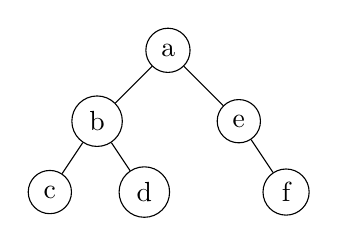
\begin{tikzpicture}[scale=0.6]
      \tikzstyle{every node}=[circle,draw]
      \tikzstyle{level 1}=[sibling distance=3cm]
      \tikzstyle{level 2}=[sibling distance=2cm]
      \node at (0,0) {a} 
      child {node{b} child {node{c}} child {node{d}}} 
      child {node{e} child [fill=none] {edge from parent[draw=none]} child {node{f}} };
    \end{tikzpicture}
  \end{figure}
  
  利用以上类和函数,编写程序构造该二叉树,实现其层序遍历和中序遍历,并写出运行结果。
  \end{enumerate}
\item (15分)~ 给定一串数~\lstinline{53, 24, 91, 88, 34, 71, 44, 18},
  \begin{enumerate}
  \item (5分)~编写无序列表的顺序查找函数:
    \begin{lstlisting}
def sequentialSearch(alist, item):
    pos = 0
    found = False
    ...          
    return found
    \end{lstlisting}
  \item (5分)~以图示+说明的方式阐述无序列表的归并排序算法,或直接编写归并排序函数:
    \begin{lstlisting}
def mergeSort(alist):
    ...      
    \end{lstlisting}
    \item (5分)~编写代码,查找\lstinline{88}是否存在,并用归并算法对其排序。
  \end{enumerate}
\item 
\end{enumerate}



\end{CJK}
\end{document}
